\documentclass[DM,authoryear,toc]{lsstdoc}
% lsstdoc documentation: https://lsst-texmf.lsst.io/lsstdoc.html
\input{meta}

% Package imports go here.
\usepackage{comment}
\usepackage{datetime}
\usepackage{microtype}


% Local commands go here.
\newcommand{\microarcsec}{$\mu$as\xspace}
\interfootnotelinepenalty=10000
\setcounter{secnumdepth}{3}

%If you want glossaries
%\input{aglossary.tex}
%\makeglossaries

\title{Rubin Observatory Processing of Gravitational Wave TOO Data in the Early Operations Era}

% Optional subtitle
% \setDocSubtitle{A subtitle}

\input{authors}

\setDocRef{RTN-008}
\setDocUpstreamLocation{\url{https://github.com/rubin-observatory/rtn-008}}
\setDocDOI{10.71929/rubin/2997564}

% Update if the document has non-trivial revisions.
\date{2022-08-03}

% Optional: name of the document's curator
% \setDocCurator{The Curator of this Document}


% Change history defined here.
% Order: oldest first.
% Fields: VERSION, DATE, DESCRIPTION, OWNER NAME.
% See LPM-51 for version number policy.
\setDocChangeRecord{%
  \addtohist{}{2019-12-16}{Initial draft version.}{Eric Bellm}
  \addtohist{}{2020-09-20}{Moved from opstn-002 to rtn-008.}{Leanne Guy}
  \addtohist{}{2022-08-03}{Revised throughout.}{Eric Bellm}
  \addtohist{}{2025-10-05}{Add DOI}{Tim Jenness}
}


\begin{document}

\setDocAbstract{%
Since the watershed discovery of an electromagnetic counterpart to the LIGO/VIRGO gravitational wave source GW170817, multi-messenger astrophysics has emerged as a major area of strategic focus for the NSF. Rubin Observatory’s depth, survey speed, and data management systems will make it a key asset in the search for EM counterparts. Exploiting this capability during the phases of Rubin commissioning and early operations that coincide with GW observing run O4 may require special actions, however. We discuss potential approaches to data access, template building, and special data processing.
}


% Create the title page.
\maketitle
% Frequently for a technote we do not want a title page  uncomment this to remove the title page and changelog.
% use \mkshorttitle to remove the extra pages

% ADD CONTENT HERE
% You can also use the \input command to include several content files.
\section{Scientific, Technical, and Programmatic Context}

The first binary neutron star merger detected in gravitational waves, GW170817, was detected at the end of observing run O2 \citep{2017PhRvL.119p1101A} along with coincident gamma-rays \citep{2017ApJ...848L..13A}.
It was rapidly localized by many groups of electromagnetic (EM) observers \citep{2017ApJ...848L..12A}, enabling an unprecedented followup campaign.

Despite this initial success, intense followup of more than a dozen neutron-star-involved mergers in observing run O3 did not yield a credible electromagnetic counterpart \citep[e.g.,][]{2020ApJ...905..145K, 2022ApJ...927...50R, 2022MNRAS.509.3427D}.
These results suggested that deeper optical surveys are needed in order to identify EM counterparts to these events \citep[e.g.,][]{2020MNRAS.492..863C, 2021MNRAS.504.1294S}.

Given Rubin's major improvement in depth and survey speed relative to current facilities,
this scenario raises substantial community and agency expectations for the Rubin Observatory.
There is little doubt that Rubin can play a central role in identifying significant samples of EM counterparts to GW sources.

Rubin's strengths will become increasingly important in later GW observing runs:
as KAGRA and LIGO-India come online, GW spatial localizations will improve to $\sim$tens of square degrees, lessening the need for extremely wide-field instruments to tile major fractions of the sky \citep{2022ApJ...924...54P}.
However, as the GW interferometers become more sensitive the GW sources detected will be farther away, making already-faint EM counterparts even fainter.

There will certainly be other EM followup programs active in the Southern Hemisphere, including the new BlackGEM array as well as community programs with DECam.
However, Rubin is capable of making the definitive measurements, delivering high-impact early science along with another major NSF facility in an area of NSF strategic priority\footnote{``Windows on the Universe:'': \url{https://www.nsf.gov/news/special_reports/big_ideas/universe.jsp}}.

One challenge remains: the current timeline for future LIGO/Virgo/KAGRA observing runs (Figure \ref{fig:scenarios}) calls for only the end of observing run O4 to overlap with the Rubin commissioning period\footnote{See \url{https://www.lsst.org/about/project-status} for current estimates.}.
In this period prior to the first LSST data release (DR1), alert production will not be running at full volume nor full fidelity.
Moreover, after O4 there will be a long, two-year period of downtime (until 2026+) for upgrades to the GW interferometers.
Accordingly, O4 provides a key opportunity to commission Rubin's TOO capability as well as deliver important early science despite the technical challenges.

\begin{figure}
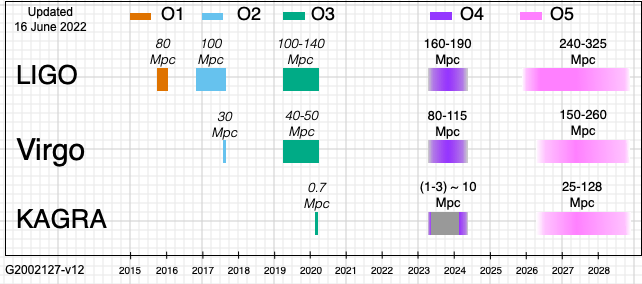
\includegraphics[width=\textwidth]{figures/LVK_run_plan_220615.png}
\caption{Projected observing scenarios for LIGO, Virgo, and KAGRA.  Retrieved 2022-07-22 from
\url{https://www.ligo.org/scientists/GWEMalerts.php}.
	\label{fig:scenarios}}
\end{figure}

The Survey Cadence Optimization Committee (SCOC\footnote{\url{https://www.lsst.org/content/charge-survey-cadence-optimization-committee-scoc}}) is resolving the relevant TOO survey strategy questions, which are outside the scope of this document\footnote{We note that the realities of the LSST data in this timeframe suggest some constraints on observing strategy:
Given the incompleteness of solar system catalogs, TOO observations should ensure two or more observations separated by an interval sufficient to reject main belt asteroids (minimally, 20 minutes, but larger separations would better capture the expected intranight temporal evolution of kilonovae).
Since there will be minimal variability history, obtaining near-simultaneous exposures in at least two bands will enable searches for sources with extreme colors.
These are consistent with the observing strategies proposed by \citet{2018arXiv181204051M} and \citet{2022ApJS..260...18A}.}
\citeds{TSTN-035} describes technical handling of TOO triggers by the Rubin scheduler.

This document asks what steps Rubin can take to maximize the scientific value of any GW TOO observations undertaken in the early operations era (defined as the time before DR1, when Data-Release templates are available for all or most of the sky; see \citeds{RTN-011}), with a particular emphasis on data processing, data products, and data availability.

Alerts are LSST's real-time data product.
In the commissioning and early operations era,
templates will not be available in many areas, and hence standard alert processing cannot be used to disseminate candidates.
Where LSST templates exist in the area to be covered, standard LSST processing can proceed as normal (subject to the caveats described in \citeds{DMTN-065}), and community alert brokers will provide community access to 60-second latency alerts from the TOO observations.

Given the potentially high impact of the science, its visibility in the community, and importance to the NSF, we suggest that the project plan for special handling of GW TOO observations in the commissioning and early operations era.

\section{Constraints} \label{sec:constraints}

Rubin's automated Alert Production relies on coadded templates generated from prior LSST images.
Given the early stage of Rubin commissioning during O4, limited on-sky time means it is probable that many LVK triggers will occur in sky areas Rubin has never imaged before.
Without templates, then, fully automated, survey-grade Alert Production will not be possible.
Accordingly, custom processing will be required in order to generate timely and useful data products.
Followup observations in the first 24 hours are among the most critical for identifying EM counterparts and constraining progenitor scenarios.

Raw and processed LSST images are initially embargoed in both commissioning and operations.
This precludes simply releasing the TOO images for community processing.
Instead, timely custom processing of TOO data must be performed by Rubin staff (\S \ref{sec:processing}).

We assume that any triggers would be on relatively well-localized GW sources (a few LSST pointings), and so this additional data processing is well within operational compute margins.

\section{Recommendations}

\subsection{Conduct incremental template building} \label{sec:templates}

Standard alert processing provides the most rapid dissemination of candidate counterparts from TOO observations with the least operational burden, but it requires the existence of template images from prior LSST observations.
Timely generation of ``incremental'' templates as commissioning and early operations proceed will thus improve the likelihood that a TOO could be processed with standard Alert Production.
In this scenario new templates are regularly generated throughout the year whenever sufficient imaging becomes available in sky areas and filters without templates.
Rubin intends to generate templates incrementally from commissioning and early operations data \citedsp{RTN-011}.

Additionally, evidence of variability prior to the GW trigger provides one of the most effective ways to rule out unassociated sources in the GW localization region \citep[e.g.,][]{2019GCN.24223....1C, 2019GCN.26430....1S}.
At LSST depths there will be many unrelated events, and little recent prior imaging of sufficient depth from other surveys that can constrain the explosion date.

In the steady state survey, LSST's own history will provide substantial filtering: simply selecting \DIAObjects created after the trigger will exclude most unrelated contaminants.
In early operations, however, this history will not be available, so not only distant supernovae but also variable stars and AGN will confound efforts to identify plausible GW counterparts.

For this reason it will be very helpful for Rubin to have reliable standard image differencing processing---and hence history---as soon as is practical, providing further support for the planned incremental template building.
While custom processing and association could be used to derive this history (\S \ref{sec:processing}) it would require substantial additional effort relative to LSST's standard processing.

If TOO observations are expected to be conducted in a subset of LSST's filters, any observations intended to maximize template coverage could prioritize obtaining images in those bands.

\subsection{Conduct bespoke image differencing on-project} \label{sec:processing}

We suggest that the Rubin commissioning and operations teams devote specific effort to custom manual processing and analysis of TOO observations.
This processing is necessary for the community to be able to utilize the Rubin observations in a timely manner (\S \ref{sec:constraints}): when pre-existing templates are not available for the fields to be observed (\S \ref{sec:templates}), no regular data products will be automatically available.

In this scenario, an on-call Rubin team would undertake a best-effort activity to produce direct image sources, \DIASources, and/or \DIAObjects (if possible) for the TOO observations through manual processing of the TOO data.
The goal would not be to perform scientific analysis\footnote{though team members would not be precluded from doing so later} but to rapidly report reliable results to the community.
The team would use its judgment to undertake custom processing to enable the rapid identification of plausible counterparts.
This processing might include image-to-image differencing using prior LSST data, on-the-fly generation of new templates, or various flavors of forced photometry.

While it might be possible to generate functional alert packets to forward to community alert brokers, the team would also likely report results via other channels, in particular the GCN Circulars used by the broader EM/GW community.
As an extremely time-sensitive, alert-like product these results would be made world-public immediately.

Rubin's TOOs will be highly visible, highly scrutinized observations, and so it will be valuable to have data processing performed by the experienced Rubin team under the Rubin imprimatur.
Successful execution of such processing will require a specialized team that will agree to be on-call in case of TOO triggers.
This team would consist primarily of Rubin personnel but could include members of the commissioning team with relevant expertise (emphasizing again that the purpose of this activity is data processing, not science analysis).

It will be crucial to develop and rehearse procedures in advance to clarify authority, responsibility, and communications channels.
In developing these procedures it would be useful to consult with the operations of other public facilities conducting EM/GW followup, such as \textit{Swift} and \textit{Fermi}.

During O4 the on-call team should be activated even in cases when templates exist for the TOO observations.
In this case manual processing might not be required, but the team would perform detailed QA of the alerts produced by the standard pipeline and report any problems with the automated analysis to the community via GCN.

We assume that TOO observations are relatively uncommon in this period (restricted to no more than 1--2 triggers/month, on average, perhaps) such that the impacts on on-call staff are tolerable.
Criteria to trigger during high priority commissioning activities will be worked out with the commissioning team and project management.


\appendix
% Include all the relevant bib files.
% https://lsst-texmf.lsst.io/lsstdoc.html#bibliographies
\section{References} \label{sec:bib}
\renewcommand{\refname}{} % Suppress default Bibliography section
\bibliography{local,lsst,lsst-dm,refs_ads,refs,books}

% Make sure lsst-texmf/bin/generateAcronyms.py is in your path
\section{Acronyms} \label{sec:acronyms}
\addtocounter{table}{-1}
\begin{longtable}{p{0.145\textwidth}p{0.8\textwidth}}\hline
\textbf{Acronym} & \textbf{Description}  \\\hline

 &  \\\hline
AGN & active galactic nuclei \\\hline
DM & Data Management \\\hline
DM-SST & DM System Science Team \\\hline
DMTN & DM Technical Note \\\hline
DR1 & Data Release 1 \\\hline
GCN & GRB Coordinates Network \\\hline
GW & Gravitational Wave \\\hline
LDO & LSST Document Operations (Document Handle) \\\hline
LIGO & Laser Interferometer Gravitational-Wave Observatory \\\hline
LSE & LSST Systems Engineering (Document Handle) \\\hline
LSR & LSST System Requirements; LSE-29 \\\hline
LSST & Legacy Survey of Space and Time (formerly Large Synoptic Survey Telescope) \\\hline
NSF & National Science Foundation \\\hline
OPS & Operations \\\hline
QA & Quality Assurance \\\hline
RTN & Rubin Technical Note \\\hline
SST & Subsystem Science Team \\\hline
\end{longtable}

% If you want glossary uncomment below -- comment out the two lines above
%\printglossaries





\end{document}
